\providecommand{\zZ}{\hskip 3.6pt plus1.2pt minus0.8pt}
\providecommand{\McQ}{\fontfamily{cwM}\fontseries{2}\selectfont}
\providecommand{\MbQ}{\fontfamily{cwM}\fontseries{1}\selectfont}
\providecommand{\zz}{\hskip 0.6pt plus0.2pt minus0.1pt\ignorespaces}
\providecommand{\MdQ}{\fontfamily{cwM}\fontseries{3}\selectfont}
\catcode+252=1 \catcode+253=2 \catcode+254=0 \catcode+251=4
\providecommand{\MmQ}{\fontfamily{cwM}\fontseries{12}\selectfont}
\providecommand{\z}{\hskip 0.0pt plus0.2pt minus0.1pt}
\providecommand{\Z}{\hskip 1.2pt plus0.4pt minus0.2pt}
\providecommand{\cH}{\char}
\providecommand{\MjQ}{\fontfamily{cwM}\fontseries{9}\selectfont}
\documentclass[a4paper,12pt]{article}
\usepackage{ amssymb }
\usepackage{ stmaryrd }
\usepackage{ dsfont }
\usepackage{amsmath}
\usepackage{mathtools} 
\newcommand{\tabincell}[2]{\begin{tabular}{@{}#1@{}}#2\end{tabular}} %{\McQ\cH91}{\MbQ\cH143}{\MaQ\cH113}{\MbQ\cH35}{\MaQ\cH132}{\MfQ\cH178}{\McQ\cH87}{\MaQ\cH223}{\MbQ\cH224}
\usepackage{textcomp}
\renewcommand{\baselinestretch}{1.5} % 5 linespace
%\usepackage{MinionPro} %{\MiQ\cH28}{\MfQ\cH220}{\MiQ\cH116}{\MbQ\cH143}{\MbQ\cH61}{\MbQ\cH224}{\MbQ\cH237}{\McQ\cH76}{\MbQ\cH100}{\MbQ\cH98}{\MaQ\cH229}{\MaQ\cH229}{\McQ\cH241}
\usepackage[utf8]{inputenc}
\usepackage{geometry}
\usepackage{graphicx,psfrag,booktabs}
\geometry{left=1in,right=1in,top=1in,bottom=1in}
\usepackage{graphicx}
\usepackage{titlesec}
\titlelabel{\thetitle.\quad} %{\MaQ\cH94}{\MbQ\cH90}section {\McQ\cH41}{\McQ\cH85}{\MbQ\cH237}{\MeQ\cH165}{\MdQ\cH168}
\usepackage{mathrsfs} %{\MaQ\cH139}{\MaQ\cH112}{\McQ\cH73}{\McQ\cH241}{\MaQ\cH229}{\MgQ\cH130}{\MeQ\cH165}{\MdQ\cH168}
%\usepackage{indentfirst}%{\McQ\cH199}{\McQ\cH229}{\McQ\cH11}{\MaQ\cH115}{\MbQ\cH143}{\MbQ\cH237}{\MbQ\cH78}{\MaQ\cH73}
\usepackage[square,numbers]{natbib}
\usepackage{xeCJK} %{\MaQ\cH50}{\MbQ\cH100}{\MaQ\cH229}{\McQ\cH241}{\McQ\cH113}{\MaQ\cH236}
\setCJKmainfont{SimSun} %{\McQ\cH227}{\McQ\cH113}{\MaQ\cH53}{\MaQ\cH50}{\MbQ\cH100}{\MaQ\cH229}{\McQ\cH241}
\bibliographystyle{unsrtnat}
\makeatletter
\def\@xfootnote[#1]{%
  \protected@xdef\@thefnmark{#1}%
  \@footnotemark\@footnotetext}
\makeatother

\title{Home Work 2\\ Machine Learning Foundations}
\author{R04323050 \\{\McQ\cH37}\z{\MbQ\cH200}\z{\MmQ\cH238}\z{\McQ\cH250}   \quad {\McQ\cH207}\z{\MdQ\cH43}\z{\MjQ\cH254}}
\date{}

\begin{document}
\maketitle
\section{}
\begin{figure}[h]
\centering
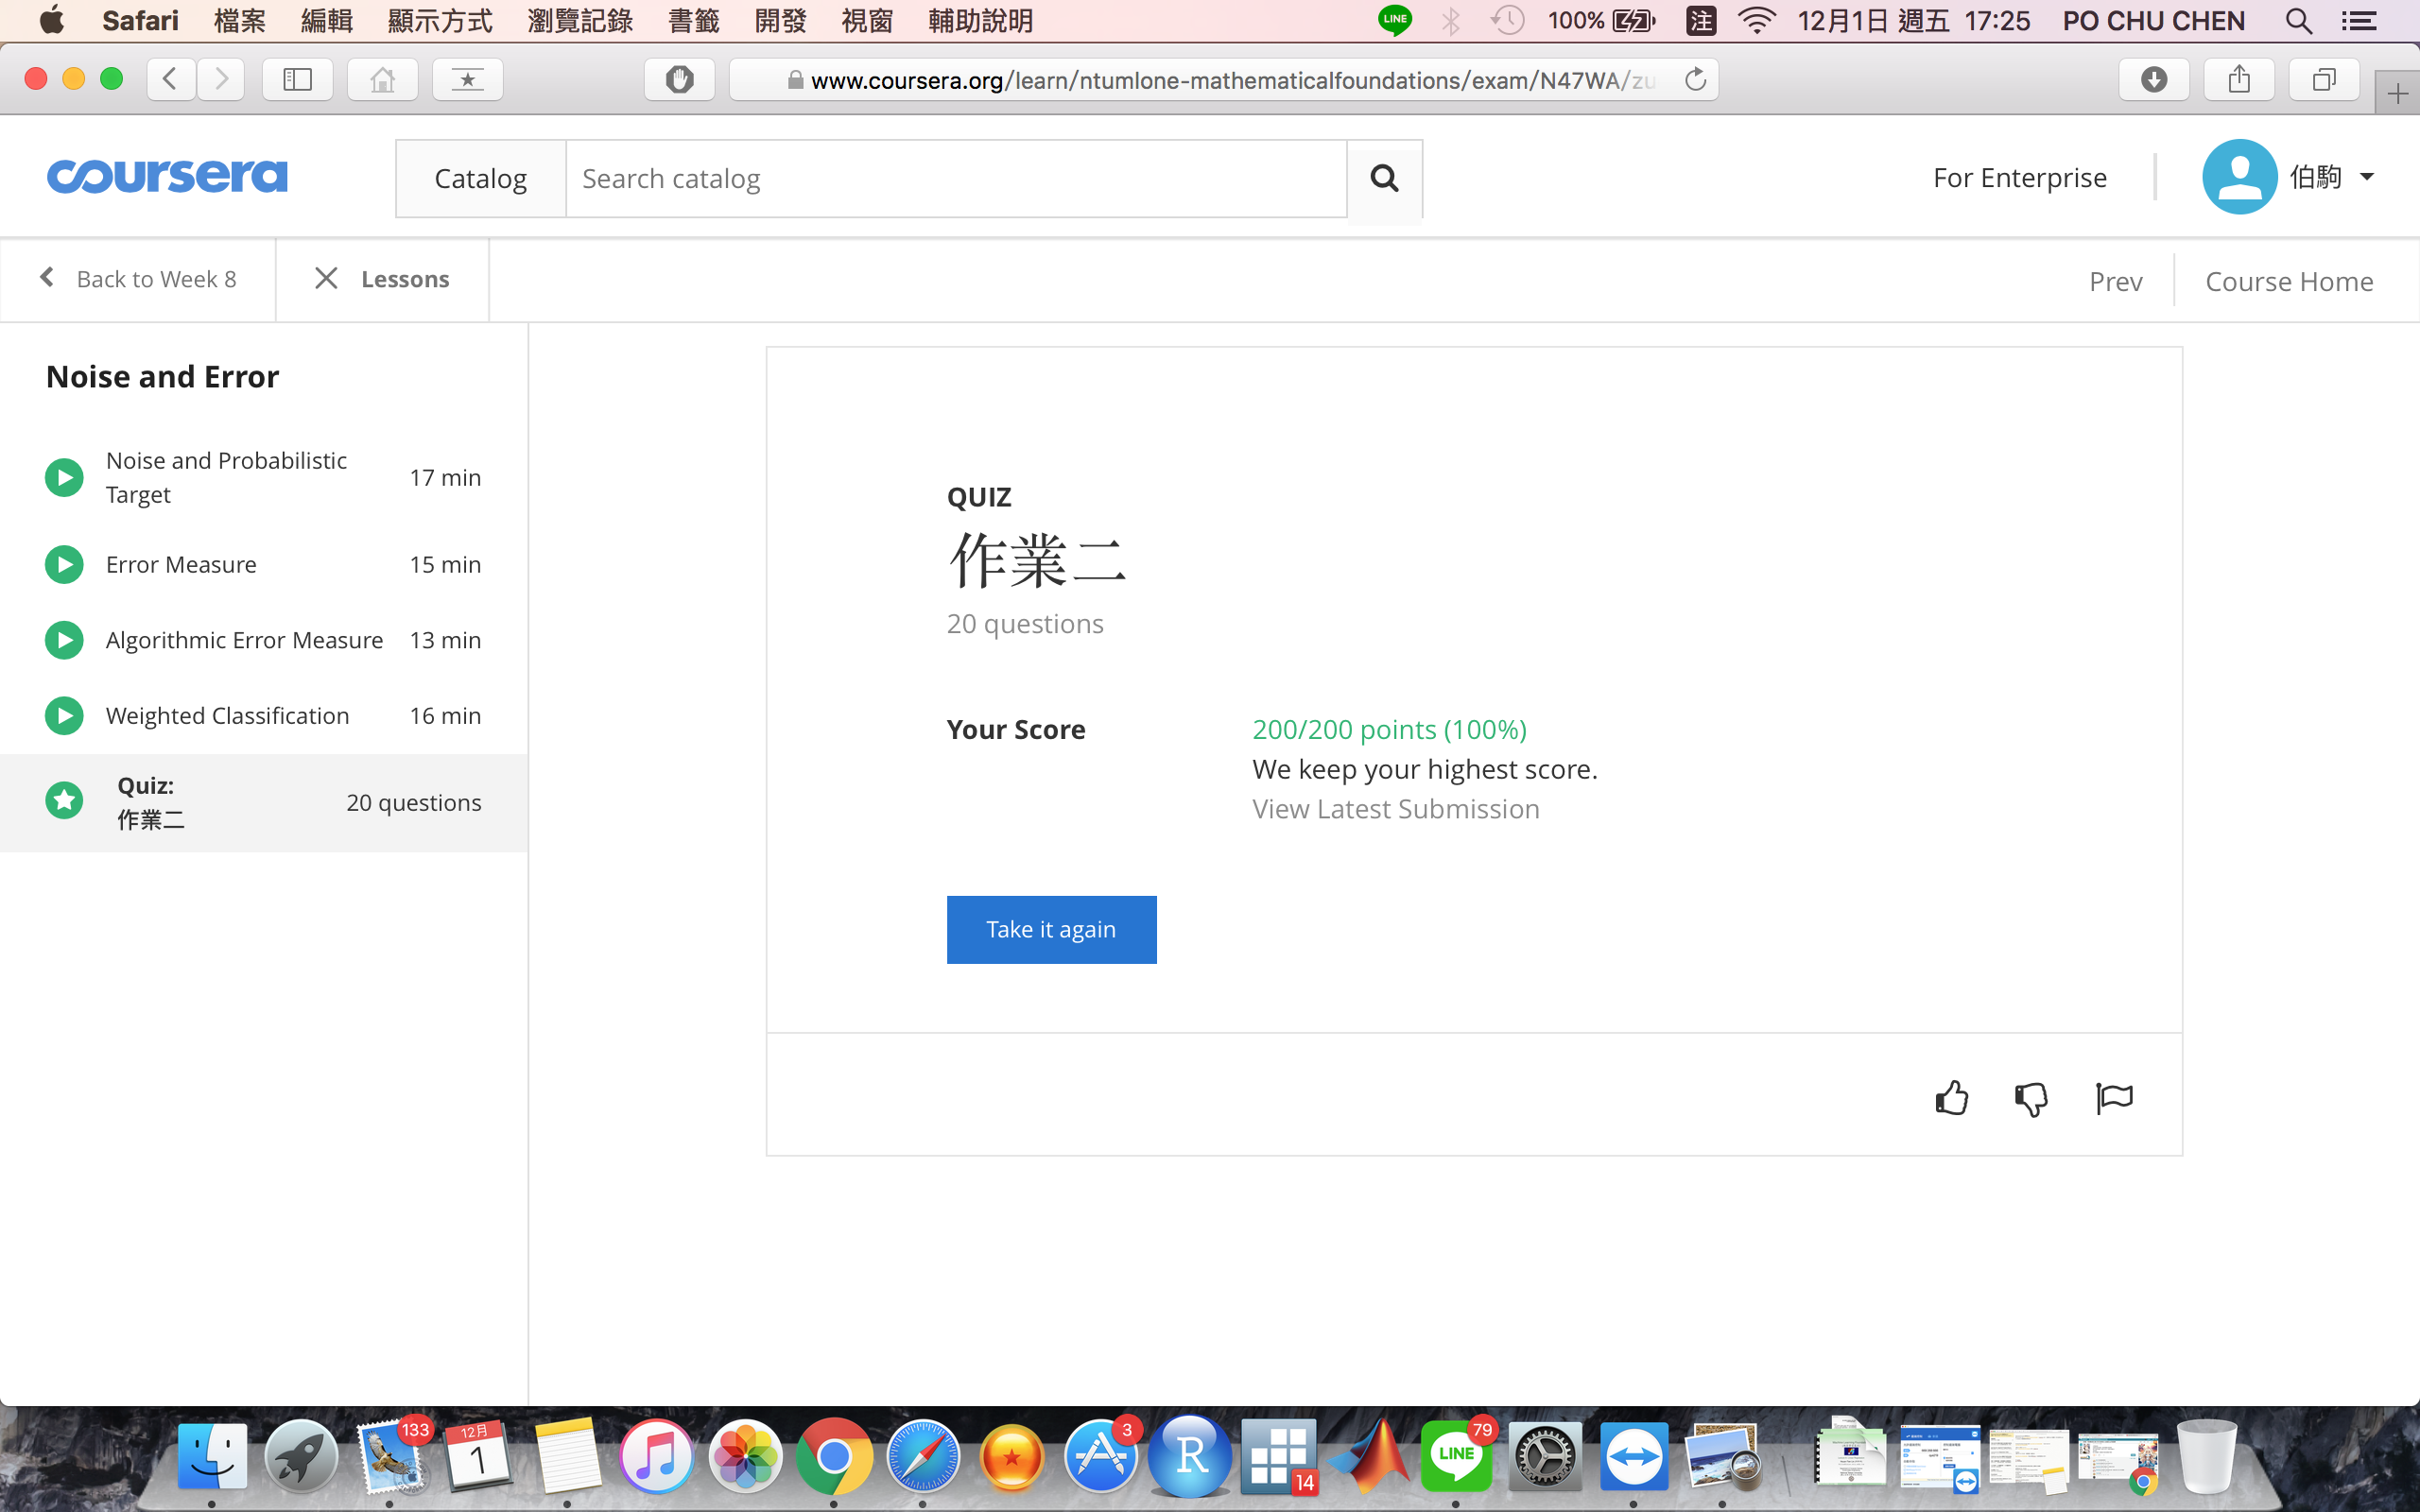
\includegraphics[scale=0.3]{Q1.png}
\end{figure}

\section{}
Positive \& Negative interval on $\mathbb{R}$. {\MaQ\cH170}\z{\McQ\cH63}\z{\MbQ\cH237}\z{\MaQ\cH150}\z{\McQ\cH200}\z{\MbQ\cH127}\z{\MaQ\cH74}\z{\MaQ\cH45}\z{\MbQ\cH56}\z{\MbQ\cH36}:\\
  \begin{minipage}{\linewidth}
      \begin{minipage}{0.45\linewidth}
\raggedright
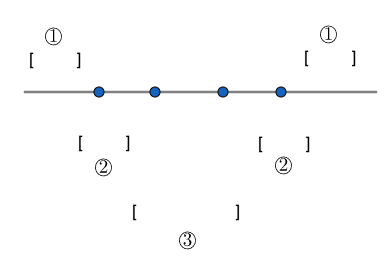
\includegraphics[scale=0.5]{Q2.png}
      \end{minipage}
      \hspace{0.05\linewidth}
      \begin{minipage}{0.45\linewidth}
      \textcircled{1}: {\MaQ\cH114}\z{\MbQ\cH209}"$-$" {\MbQ\cH67}\z{\MaQ\cH114}\z{\MbQ\cH209}"$+$"\\
      \textcircled{2}: $+-${\MbQ\cH67}$-+$\\
      \textcircled{3}: $+-+${\MbQ\cH67}$-+-$\\
      N {\MaQ\cH95}\z{\McQ\cH245}\z{\MaQ\cH50}\z{\McQ\cH200}\z{\MbQ\cH127}N-1\Z{\MaQ\cH95}\z{\McQ\cH200}\z{\MjQ\cH189}\\
      $\therefore$ $m_{\mathcal{H}}(N)=2\times(1+{{N-1}\choose{1}} + {{N-2}\choose{2}})=N^{2}-N+2$
      \end{minipage}
  \end{minipage}

\section{}
\underline{\underline{\textbf{Claim:}}} $d_{vc}(\mathcal{H})=D+1$ \\
We can observe the Hypothesis Set $\mathcal{H}$ is a D-dim PLA from the slide in lecture 2.\\
$\therefore$ By the slide in lecture 7, we've shown $d_{vc}(\mathcal{H})=D+1$ during the class.

\section{}
"Triangle Waves" Hypothesis Set in $\mathbb{R}$:\\
\begin{center}
$\mathcal{H}=\left \{   h_{\alpha}  \lvert \quad h_{\alpha}(x) = sgn(\left | (\alpha x) \, mod \, 4-2  \right |-1), \alpha \in \mathbb{R}     \right \}$
\end{center}
{\MbQ\cH117}\z{\MaQ\cH95}\z{\MjQ\cH85}\z{\MbQ\cH130}\z{\MbQ\cH209}$\frac{4}{\left | \alpha \right |}$ {\MbQ\cH237}\z{\McQ\cH250}\z{\McQ\cH105}\z{\MgQ\cH154}\z{\MdQ\cH131}\z{\MbQ\cH98}.\footnote{Triangle Waves Function: http://bit.ly/2nneX45}\\
$\because$ $\alpha \in \mathbb{R}$ $\therefore$ {\MjQ\cH85}\z{\MbQ\cH130}\z{\MaQ\cH170}\z{\MaQ\cH74}\z{\MaQ\cH76}\z{\MbQ\cH60}\z{\MaQ\cH252}{\MaQ\cH1}i.e $x${\MoQ\cH87}($\mathbb{R}^{1}$) {\MaQ\cH170}\z{\MaQ\cH74}\z{\McQ\cH92}\z{\McQ\cH118}\z{\MgQ\cH19}\z{\McQ\cH40}\z{\MaQ\cH126}\z{\MbQ\cH65}\z{\MbQ\cH204}\z{\McQ\cH204}\z{\MaQ\cH214}\z{\MaQ\cH95}\z{\MaQ\cH150}\z{\MeQ\cH30}, {\MbQ\cH93}$d_{vc}(\mathcal{H})=\infty$
\section{}
\underline{\underline{\textbf{Claim:}}} If $\mathcal{H}_{1} \subseteq \mathcal{H}_{2}$, then $d_{vc}(\mathcal{H}_{1}) \leq d_{vc}(\mathcal{H}_{2})$\\
Suppose $d_{vc}(\mathcal{H}) > d_{vc}(\mathcal{H}_{2})$, {\MaQ\cH134}\z{\MaQ\cH72}\z{\McQ\cH91} $\mathcal{H}_{1}$ {\MaQ\cH170}\z{\MaQ\cH74}shatter {\MbQ\cH237}inputs {\MaQ\cH95}\z{\MbQ\cH98}\z{\MjQ\cH20}\z{\McQ\cH172} $\mathcal{H}_{2}${\MbQ\cH70}\z{\MaQ\cH170}\z{\MaQ\cH74}shatter {\MbQ\cH237}inputs{\MaQ\cH1}\zZ i.e {\McQ\cH66}\z{\MaQ\cH253}\z{\MaQ\cH230}\z{\MaQ\cH202}\z{\McQ\cH248}\z{\MaQ\cH95}inputs $x$ {\MaQ\cH85}\z{\MbQ\cH41} $\mathcal{H}_{1}(x) \notin \mathcal{H}_{2}$, contradiction.($\because$ $\mathcal{H}_{1} \subseteq \mathcal{H}_{2}$, $\therefore$ $\mathcal{H}_{1}${\MbQ\cH70}\z{\McQ\cH63}\z{\MeQ\cH68}\z{\MbQ\cH223}\z{\MbQ\cH222}\z{\MbQ\cH237}dichotomies,$\mathcal{H}_{2}${\MaQ\cH54}\z{\McQ\cH183}\z{\McQ\cH98}\z{\McQ\cH63}\z{\MeQ\cH68}\z{\MbQ\cH223}\z{\MaQ\cH124})\\
Hence, $d_{vc}(\mathcal{H}) \leq d_{vc}(\mathcal{H}_{2})$


\section {}
By Q.15 on Couresa: \underline{\underline{\textbf{Claim:}}} $\max \left \{   d_{vc} (\mathcal{H}_{k})   \right \}_{k=1}^{K} \leq d_{vc}(\displaystyle \bigcup_{k=1}^{K}\mathcal{H}_{k} ) \leq K-1+ \displaystyle \sum_{k=1}^{K} d_{vc}(\mathcal{H}_{k})$ \\
\textbf{Left:}
\begin{minipage}[t]{0.9\linewidth}
{\McQ\cH113}$\mathcal{H}_{1}, \mathcal{H}_{2},...,\mathcal{H}_{K}$ {\MbQ\cH70}\z{\McQ\cH63}\z{\MeQ\cH68}shatter {\MbQ\cH237}\z{\MbQ\cH124}\z{\MaQ\cH215}inputs {\MaQ\cH95}\z{\MbQ\cH98}\z{\MbQ\cH209}$N$, {\MaQ\cH134}$\displaystyle \bigcup_{k=1}^{K} \mathcal{H}_{k}${\MaQ\cH54}\z{\McQ\cH66}\z{\MaQ\cH253}\z{\McQ\cH63}\z{\MeQ\cH68}shatter $N${\MaQ\cH95}inputs:\\
Suppose not, i.e suppose $d_{vc}(\displaystyle \bigcup_{k=1}^{K} \mathcal{H}_{k})=N-1$, {\McQ\cH165}\z{\MaQ\cH60}$\mathcal{H}_{1}, \mathcal{H}_{2},...,\mathcal{H}_{K}${\McQ\cH58}\z{\McQ\cH213}\z{\McQ\cH150}\z{\MaQ\cH86}\z{\MbQ\cH70}\z{\MbQ\cH36}\z{\MbQ\cH65}\z{\MbQ\cH237}Hypothesis Set {\MbQ\cH124}\z{\MaQ\cH214}\z{\MdQ\cH201}\z{\McQ\cH63}shatter  $N-1${\MaQ\cH95}inputs, {\MaQ\cH72}\z{\McQ\cH91}\z{\McQ\cH165}\z{\MaQ\cH53}\z{\MaQ\cH50}\z{\MbQ\cH70}\z{\McQ\cH63}shatter {\MbQ\cH124}\z{\MaQ\cH214}\z{\MbQ\cH237}inputs {\MaQ\cH54}\z{\MdQ\cH201}\z{\MbQ\cH125}\z{\MaQ\cH131}$N-1${\MaQ\cH95}, contradiction.\\
Hence, $\max \left \{   d_{vc} (\mathcal{H}_{k})   \right \}_{k=1}^{K} \leq d_{vc}(\displaystyle \bigcup_{k=1}^{K}\mathcal{H}_{k} )$
\end{minipage}
\\
\textbf{Right:}
\begin{minipage}[t]{0.9\linewidth}
{\MaQ\cH99}\z{\McQ\cH113}\z{\MbQ\cH219}\z{\MaQ\cH202}\z{\MdQ\cH201}\z{\MbQ\cH127} $\mathcal{H}_{1}, \mathcal{H}_{2}$ {\McQ\cH165}\z{\MaQ\cH115}\z{\McQ\cH7}Hypothesis Sets,$\mathcal{H}_{1}${\MbQ\cH117}\z{\MfQ\cH122}\z{\MbQ\cH19}\z{\McQ\cH222}\z{\MaQ\cH44}\z{\MbQ\cH70}\z{\MbQ\cH127}\z{\MbQ\cH237}\z{\McQ\cH245}\z{\MbQ\cH166}\z{\McQ\cH233}\z{\MbQ\cH209}$+1$; $\mathcal{H}_{2}${\MbQ\cH117}\z{\MfQ\cH122}\z{\MbQ\cH19}\z{\McQ\cH222}\z{\MaQ\cH44}\z{\MbQ\cH70}\z{\MbQ\cH127}\z{\McQ\cH245}\z{\MbQ\cH166}\z{\McQ\cH233}\z{\MbQ\cH209}$-1$, {\MaQ\cH134}\z{\MbQ\cH66}\z{\MaQ\cH98}\z{\MbQ\cH248}\z{\McQ\cH173}$d_{vc}(\mathcal{H}_{1})=0$ \& $d_{vc}(\mathcal{H}_{2})=0$,$d_{vc}(\mathcal{H}_{1} \cup \mathcal{H}_{2})=1${\MaQ\cH1}\\
$\therefore$ {\MbQ\cH42}Coursera Q.15\Z{\MbQ\cH237}\z{\McQ\cH178}\z{\McQ\cH225}\z{\MaQ\cH50},$d_{vc}(\mathcal{H}_{1} \cup \mathcal{H}_{2})=1$, $\displaystyle \sum_{k=1}^{K} d_{vc}(\mathcal{H}_{k})=0$.\\
Hence, $d_{vc}(\mathcal{H}_{1} \cup \mathcal{H}_{2})=1 \leq 2-1+0= K-1+\displaystyle \sum_{k=1}^{K} d_{vc}(\mathcal{H}_{k})=0${\MbQ\cH65}\z{\McQ\cH13}{\MaQ\cH1}\zZ
\end{minipage}
\\
Therefore, $\max \left \{   d_{vc} (\mathcal{H}_{k})   \right \}_{k=1}^{K} \leq d_{vc}(\displaystyle \bigcup_{k=1}^{K}\mathcal{H}_{k} ) \leq K-1+ \displaystyle \sum_{k=1}^{K} d_{vc}(\mathcal{H}_{k})$.\\
Now let $\mathcal{H}_{1}$ be positive-ray hypothesis set and $\mathcal{H}_{2}$ be negative-ray hypothesis set. By the slides in lecture 5, we know:
\begin{minipage}[t]{0.9\linewidth}
$m_{\mathcal{H}_{1}}(N)=N+1, \quad d_{vc}(\mathcal{H}_{1})=1$ \\
$m_{\mathcal{H}_{2}}(N)=N+1, \quad d_{vc}(\mathcal{H}_{2})=1$
\end{minipage}
\\
$\therefore$ $\max \left \{   d_{vc} (\mathcal{H}_{k})   \right \}_{k=1}^{2}=1 \leq d_{vc}(\mathcal{H}_{1} \cup \mathcal{H}_{2} ) \leq K-1+ \displaystyle \sum_{k=1}^{2} d_{vc}(\mathcal{H}_{k})=2-1+2=3$\\
$\Rightarrow$ $1 \leq d_{vc}(\mathcal{H}_{1} \cup \mathcal{H}_{2} ) \leq 3$.\\
Also, we know the hypothesis set $\mathcal{H}_{1} \cup \mathcal{H}_{2}$ is actually the 1-d perceptron. Hence,          $m_{\mathcal{H}_{1} \cup \mathcal{H}_{2}}(N)=2N$   and $d_{vc}({\mathcal{H}_{1} \cup \mathcal{H}_{2}})=2$ by the slides in lecture 5 and 7, which holds in the above inequality.

\section{}
$x$ is generated by a uniform distribution in [-1,1].\\
  \begin{minipage}{\linewidth}
      \begin{minipage}{0.6\linewidth}
\raggedright
     \begin{tabular}{c|cc|c}
      & $\theta $ &  $s$   & \tabincell{c}{  {\McQ\cH227}\z{\MgQ\cH191}\z{\MjQ\cH152}\z{\MiQ\cH207}\z{\MhQ\cH48}$\mu=P(h \neq f)$ \\ $=P(s\cdot sgn(x-\theta) \neq sgn(x))$   } \\ \hline
\textcircled{1} & > 0 & $+1$ & $P(sgn(x-\theta) \neq sgn(x))=\theta \times \frac{1}{2}$\\ \hline
\textcircled{2} & > 0 & $-1$ &  \tabincell{c}{ $P(-sgn(x-\theta) \neq sgn(x))$ \\$=[1+(1-\theta)]\times \frac{1}{2}=1-\frac{\theta}{2}$  } \\ \hline
\textcircled{3} & < 0 & $+1$ & $P(sgn(x-\theta) \neq sgn(x))=-\theta \times \frac{1}{2}$\\ \hline
\textcircled{4} & < 0 & $-1$ &  \tabincell{c}{  $P(-sgn(x-\theta) \neq sgn(x))$ \\ $=[1+(1+\theta)]\times \frac{1}{2}=1+\frac{\theta}{2}$  } \\

\end{tabular}

      \end{minipage}
      \hspace{0.05\linewidth}
      \begin{minipage}{0.4\linewidth}
 
      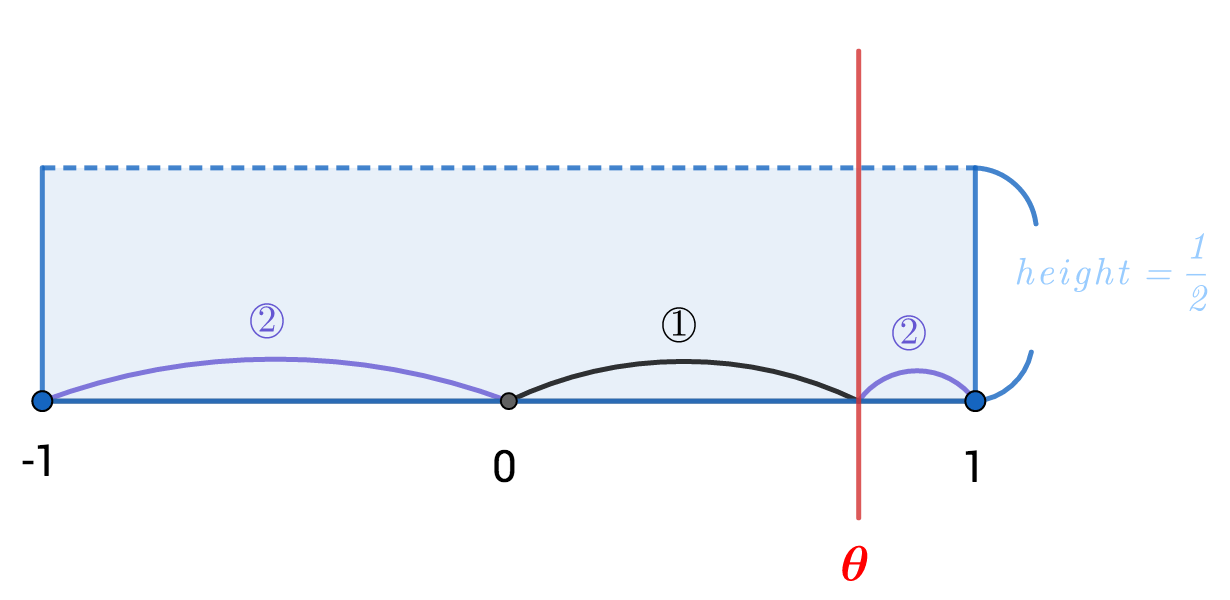
\includegraphics[scale=0.3]{Q71.png}
      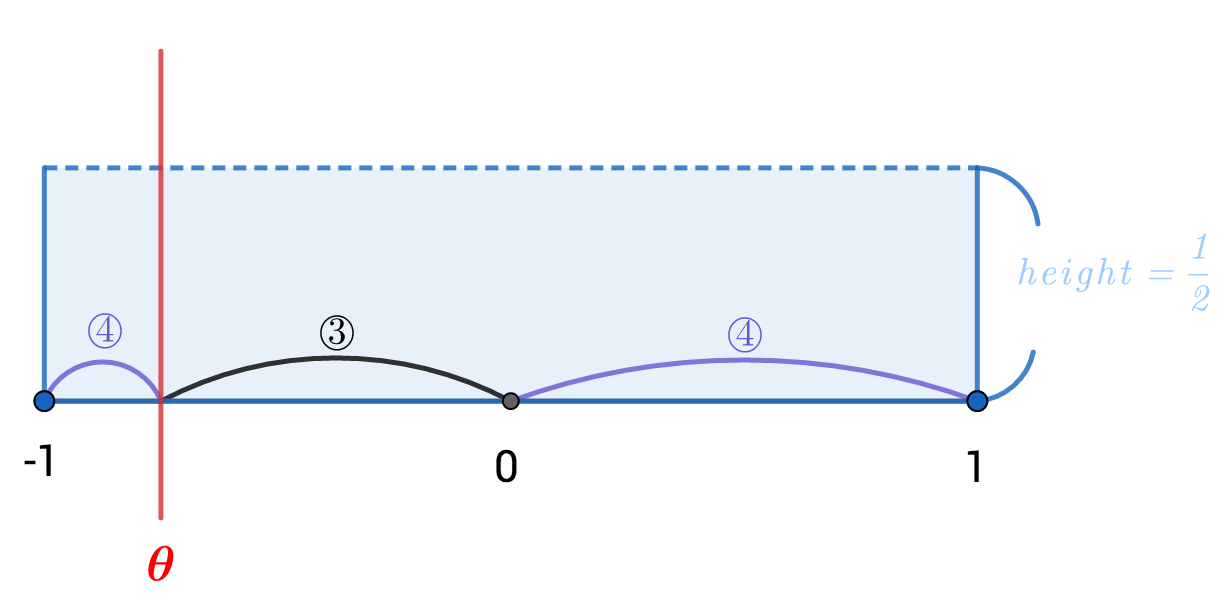
\includegraphics[scale=0.3]{Q72.png}
      \end{minipage}
  \end{minipage}
{\MhQ\cH227}\z{\MaQ\cH175}\textcircled{1} {\MaQ\cH2}\textcircled{2} {\MaQ\cH2}\textcircled{3} {\MaQ\cH2}\textcircled{4} : 
$\mu=$  
$\begin{cases}
\left | \theta \right | \times \frac{1}{2} \text{\quad if $s=+1$} \\
1-\frac{\left | \theta \right |}{2} \text{\quad if $s=-1$}
\end{cases}$
$\overset{\text{{\MaQ\cH115}\z{\McQ\cH245}\z{\MbQ\cH31}}}{\Longrightarrow}\mu= \frac{1}{2}+ (\frac{|\theta|-1}{2})\times s${\MaQ\cH1}\zZ \footnote{Let $\mu=a \cdot s + b$. \quad  $|\theta| \times \frac{1}{2}= a+b$ \--- \textcircled{1}, $1-\frac{|\theta|}{2}=-a+b$ \--- \textcircled{2} \qquad By \textcircled{1}, \textcircled{2} $\Rightarrow$ $a=\frac{|\theta|-1}{2}, b=\frac{1}{2}$} 
\\
\begin{flalign*}
\text{By Q.1 on coursera, we know} \; E_{out}(h_{s,\theta})&=\lambda \cdot \mu + (1-\lambda) \cdot (1-\mu), \text{ where}\;  \lambda=1-0.2=0.8\\
&=0.8 \times \mu + 0.2 \times (1-\mu) \\
&=0.5 + 0.3(|\theta|-1)\cdot s
\end{flalign*}

\section{}
  \begin{minipage}{\linewidth}
      \begin{minipage}{0.5\linewidth}
\raggedright
         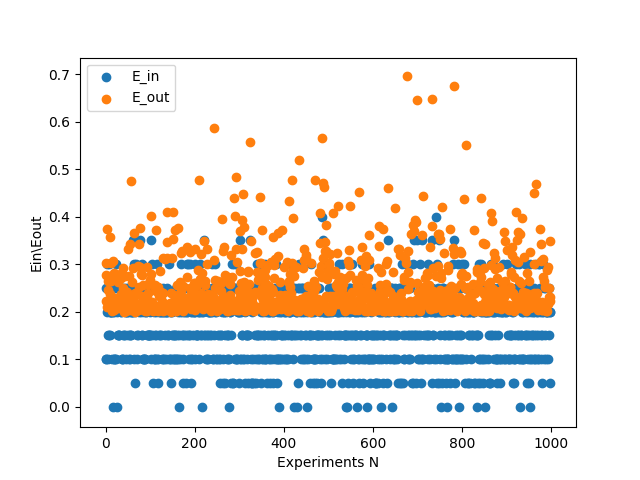
\includegraphics[scale=0.55]{Q81.png}

      \end{minipage}
      \hspace{0.05\linewidth}
      \begin{minipage}{0.4\linewidth}
        In the left figure, we can observe that the value of $E_{in}$ is at least $0.2$, which is exactly the probability of flipping noise. Intuitively, $E_{out}$ is the expectation of $\llbracket g(x) \neq f(x) \rrbracket$ out of sample, now the flipping rate is $20\%$, then the above expectation term will be at least $20\%$.    
      \end{minipage}
  \end{minipage}
 \\ 
Though we also have noise in sample of $E_{in}$, we can choose $s$ and $\theta$ to let $E_{in}$ become smaller, so $E_{in}$ could be less than $20\%$. However, the flipped $y$  for out-of-sample is followed a distribution(i.e our target funtcion) like Q.1 in coursera, which has a $20\%$ filpped rate the optimal $s$ and $\theta$ that I choose through $E_{in}$, so $E_{out}$ will be at least $20\%$. \\
\newline
  \begin{minipage}{\linewidth}
      \begin{minipage}{0.5\linewidth}
\raggedright
         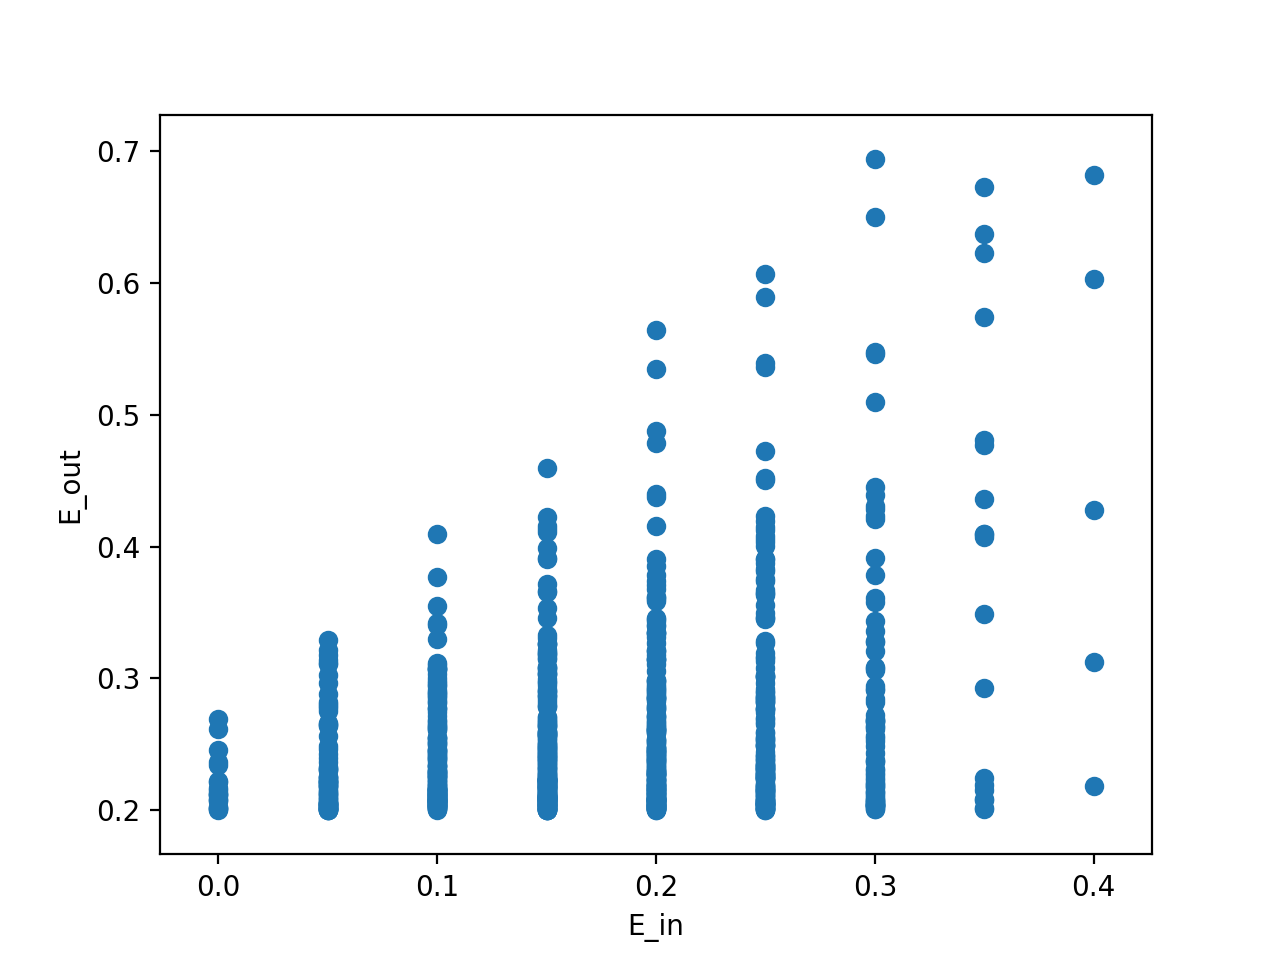
\includegraphics[scale=0.55]{Q82.png}

      \end{minipage}
      \hspace{0.05\linewidth}
      \begin{minipage}{0.4\linewidth}
       Moreover, if we put $E_{in}$ and $E_{out}$ in the same plot, we can observe that when $E_{in}$ is smaller; the variation of $E_{out}$ will also be smaller. This result corresponds to what we expect: we can let $E_{out}$ be small enough as long as we choose optimal $s$ and $\theta$ to minimize $E_{in}$. i.e Learning succeed: $E_{in} \approx E_{out}$ and $E_{in}$, $E_{out}$ are small.
      \end{minipage}
  \end{minipage}



\section{}
\underline{\textbf{Cover's Function Counting Theorem:}}\\
Let $\left \{ x^{1}, x^{2},...,x^{p} \right \}$ be vectors in $\mathbb{R}^{N}$, then the number of distinct dichotomies applied to these points that can be realized by a plane through the origin is :\\ 
\begin{center}
$C(P,N)=2\times \displaystyle \sum_{k=0}^{N-1} {{P-1}\choose{k}}$
\end{center}
{\MaQ\cH202}d-{\McQ\cH38}\z{\MbQ\cH237}PLA {\MaQ\cH50}, {\MbQ\cH66}\z{\MaQ\cH98}\z{\MbQ\cH125}\z{\MaQ\cH250}\z{\McQ\cH198}\z{\MqQ\cH167}\z{\MdQ\cH77}$w_{0}${\MaQ\cH121}\z{\MkQ\cH221}\z{\McQ\cH242}\z{\McQ\cH248}\z{\MaQ\cH95}\z{\MaQ\cH178}\z{\McQ\cH190}$x_{0}=(1,1,1,...,1)$, {\MbQ\cH224}\z{\MaQ\cH86}\z{\McQ\cH12}\z{\MbQ\cH250}\z{\MaQ\cH125}\z{\MjQ\cH189}\z{\McQ\cH40}\z{\MdQ\cH201}\z{\McQ\cH63}\z{\McQ\cH166}\z{\McQ\cH172}\z{\MaQ\cH159}\z{\McQ\cH245}\z{\MbQ\cH237}\z{\McQ\cH204}\z{\MaQ\cH132}, {\McQ\cH55}\z{\MbQ\cH27}\z{\McQ\cH50}\z{\MaQ\cH44}\z{\MaQ\cH86}\z{\McQ\cH122}\z{\MaQ\cH255}\z{\MbQ\cH117}\z{\MaQ\cH202}$\mathbb{R}^{d+1}${\MaQ\cH50}\z{\MbQ\cH237}\z{\MaQ\cH178}\z{\McQ\cH190}$\left \{ x_{1}, x_{2},...,x_{N}, x_{0} \right \}${\MaQ\cH100}\z{\McQ\cH166}\z{\McQ\cH172}\z{\MaQ\cH159}\z{\McQ\cH245}\z{\MbQ\cH237}PLA{\MaQ\cH1}\\
$\therefore$ By Cover's theorem, $m_{\mathcal{H}}(N)=C(d+1,N)=2\times \displaystyle \sum_{i=0}^{d+1-1} {{N-1}\choose{i}}=2\times \displaystyle \sum_{i=0}^{d} {{N-1}\choose{i}}$ \\
\newline
\textbf{Proof of Cover's theorem:}\footnote{Reference: http://bit.ly/2nnEtGC}\\
Denote the number of linearly separable partition by $C(P,N)$. We will find the expression for $C(P,N)$ by induction. Image first having $p$ points and then adding one more point. Now, considering the linearly separable partitions of previous $p$ points, there are two possibilities:\\
Case 1: there is a separating hyperplane for the previous $p$ points passing through the new point, in which case each such linearly separable partition of the previous $p$ points gives rise to two distinct linearly separable partitions as the hyperplane can be shifted infinitesimally to place the new point in either class. \\
Case 2: there is no separating hyperplane for the previous $p$ points passing through the new point, in which case each such linearly separable partition gives rise to only one linearly separable partition. \\
The number of linearly separable partition in Case 1 is precisely $C(P,N-1)$, because restricting the separating hyperplane to pass through a fixed point is the same as eliminating one degree of freedom and thus projecting the $p$ points to a $N-1$-dim space. This can be understood if the new point is on the $x$-axis, for example - then the hyperplane has $N-1$ axes left to work with. If the point is not on the $x$-axis, then rotate the axes of space around to get the point on the x axis, and this of course has no effect on the geometry of the problem. \\
The recursive relation:\\
$C(P+1,N)=C(P,N)+C(P,N-1)$, where$C(P,N)$ is the number of separable hyperplanes in Case 2, and $C(P,N-1)$
is the number of separable hyperplanes in Case 1.\\
\newline
Iterating the recursion once, we have \\
$C(P+1,N)=C(P-1,N)+2C(P-1,N-1)+C(P-1,N-2)$\\
\newline
Continue to iterate the recursion (twice)\\
$C(P+1,N)=C(P-2,N)+3C(P-2,N-1)+3C(P-2,N-2)+C(P-2,N-3)$\\
\newline
After $P-1$ iterations, we have\\
$C(P+1,N)={{P}\choose{0}}C(1,N)+ {{P}\choose{1}} C(1, N-1)+...+ {{P}\choose{P}} C(1, N-P)$, where $C(1,k)=2$ for all $k \leq 1$.\\
\newline
So, finally we have $C(P+1,N)=2\times \displaystyle \sum_{i=0}^{N-1} {{P}\choose{i}}$, where ${{P}\choose{i}}=0$
if $i>P$.

\medskip



\end{document}
